%!TEX root = ../thesis.tex
% ******************************* Thesis Appendix A ****************************
\ifpdf
    \graphicspath{{Appendix1/Figs/Raster/}{Appendix1/Figs/PDF/}{Appendix1/Figs/}}
\else
    \graphicspath{{Appendix1/Figs/Vector/}{Appendix1/Figs/}}
\fi

\chapter{Appendix A}

\section{Benchmarking functions}

The following is a list of synthetic functions and real datasets presented in previous works, where the goal is to evaluate Bayesian optimization algorithms. 

\begin{enumerate}
\item \citep{Garnett2013} Synthetic in-model data matching the proposed model, with $d=2, 3$, and $D=10, 20$.
\item \citep{Garnett2013} (Synthetic) Braning function, $d=2$, hidden in a higher dimensional space $D=10, 20$.
\item \citep{Garnett2013} Temperature data $D=106$ and $d=2$.
\item \citep{Garnett2013} Communities and Crime dataset $d=2$, and $D=96$. 
\item \citep{Garnett2013} Relative location of CT slices on axial axis with $d = 2$ and $D=318$. 
\item \citep{Djolonga2013} (Synthetic) Random GP samples from 2-dimensional Matern-Kernel-output, embedded within 100 dimensions
\item \citep{Djolonga2013} Gabor Filters: Determine visual stimuli that maximally excite some neurons which reacts to edges in the image.
We have $f(x) = \exp( -( \theta^T x - 1 )^2 )$. $\theta$ is of size 17x17, and the set of admissible signals is $d$.
\item \citep{Wang2013} (Synthethic) $d=2$ and $D=1*10^9$.
\item \citep{Wang2013} $D=47$ where each dimension is a parameter of a mixed integer linear programming solver.
\item \citep{Wang2013} $D=14$ with $d$ for a random forest body part classifier.
\item \citep{Tripathy}  (Synthetic) Use $d=1,10$ and $D=10$.
\item \citep{Tripathy} (Half-synthetic) Stochastic elliptic partial differential equation, where $D=100$, and an assume value for $d$ of $1$ or $2$.
\item \citep{Tripathy} Granular crystals $X \in \mathbb{R}^{1000 \times 2n_p +1}$, and $y \in \mathbb{R}^{1000}$.
\item \citep{Gardner2017} (Synthetic) Styblinski–Tang function where $D$ is freely choosable.
\item \citep{Gardner2017} (Synthetic) Michalewicz function where $D$ is freely choosable.
\item \citep{Gardner2017} (Simulated) NASA cosmological constant data where $D=9$.
\item \citep{Gardner2017} Simple matrix completion with $D=3$.
\item \citep{Rana2017} (Synthetic) Hertmann6d in [0, 1].
\item \citep{Rana2017} (Synthetic) Unnormalized Gaussian PDF with a maximum of 1 in $[-1, 1]^d$ for $D=20$ and $[-0.5, 0.5]^d$ for $D=50$
\item \citep{Rana2017} (Synthetic) Generalized Rosenbrock function $[-5, 10]^d$
\item \citep{Rana2017} Training cascade classifiers, with $D=10$ per group.
\item \citep{Rana2017} Optimizing alloys $D=13$. 
\item \citep{Li2018} (Synthetic) Gaussian mixture function
\item \citep{Li2018} (Synthetic) Schwefel's 1.2 function.
\item \citep{OptimizationTestFunctions} A list of optimiztation test functions can be found here.
\item \citep{Jamil2013} A more comprehensive list of general functions can be found here.
%\item https://github.com/automl/HPOlib2/tree/master/hpolib/benchmarks/synthetic_functions
\end{enumerate}

\section{The log-likelihood function as a function of $\tau$}
In \ref{Eq:LogLikelihoodF} I present the formula for the log-likelihood function which is a function of $W$.
In \ref{Eq:TauFunction} I show how modifying a scalar parameter $\tau$ can modify this loss.
In a combined formula, this looks as follows:

\begin{equation}
G: \tau \rightarrow F( \gamma(\tau; W_{ \text{fixed} }) )
\end{equation}
where we assume that $W_{ \text{fixed} }$ is fixed. 
To get an intuition for how smooth this function $G$ is, I randomly sample $W$ and visualize the change of $G(\tau)$ for different values of $\tau$.\\

\begin{figure}[H]
    \centering
    \begin{subfigure}[b]{0.40\textwidth}
        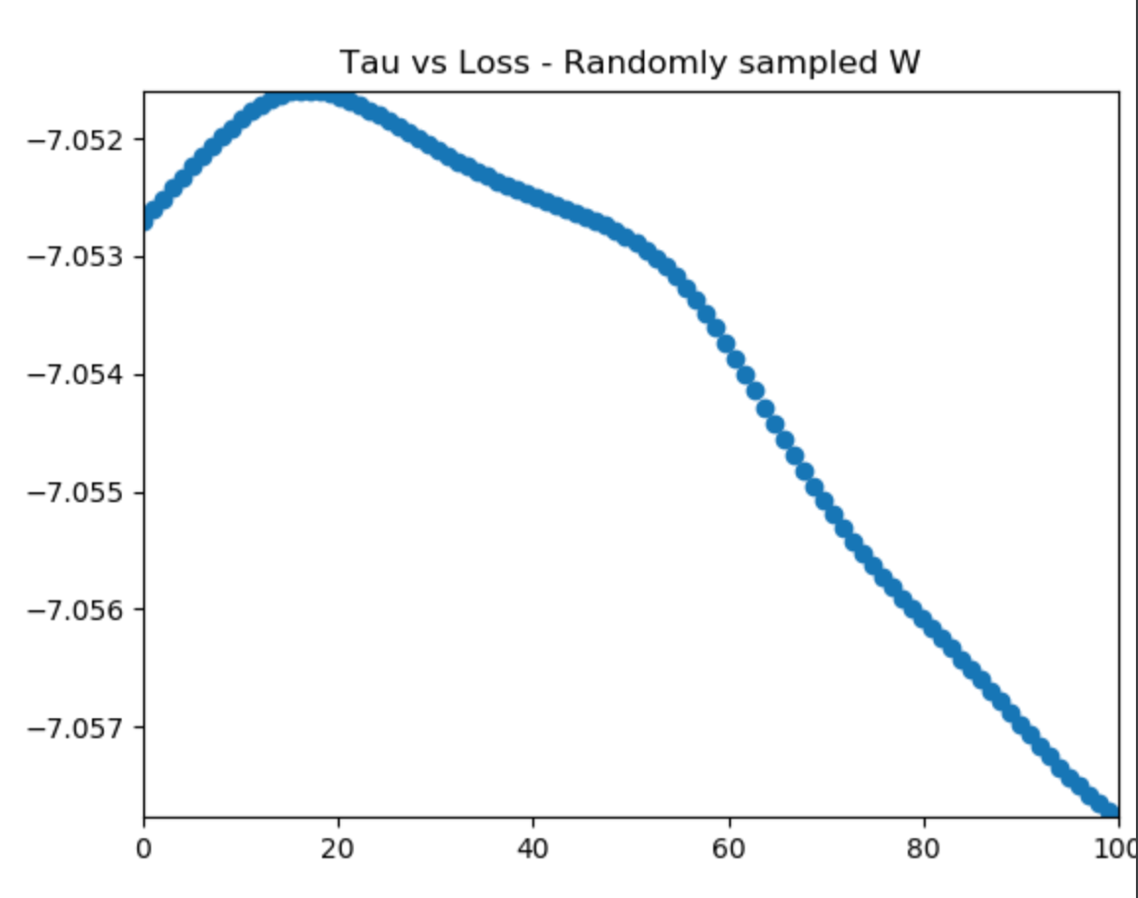
\includegraphics[width=\textwidth]{Appendix1/tau_0}
        \label{fig:gull}
        \caption{W is an orthogonal matrix}
    \end{subfigure}
    \quad
    %add desired spacing between images, e. g. ~, \quad, \qquad, \hfill etc. 
      %(or a blank line to force the subfigure onto a new line)
    \begin{subfigure}[b]{0.40\textwidth}
        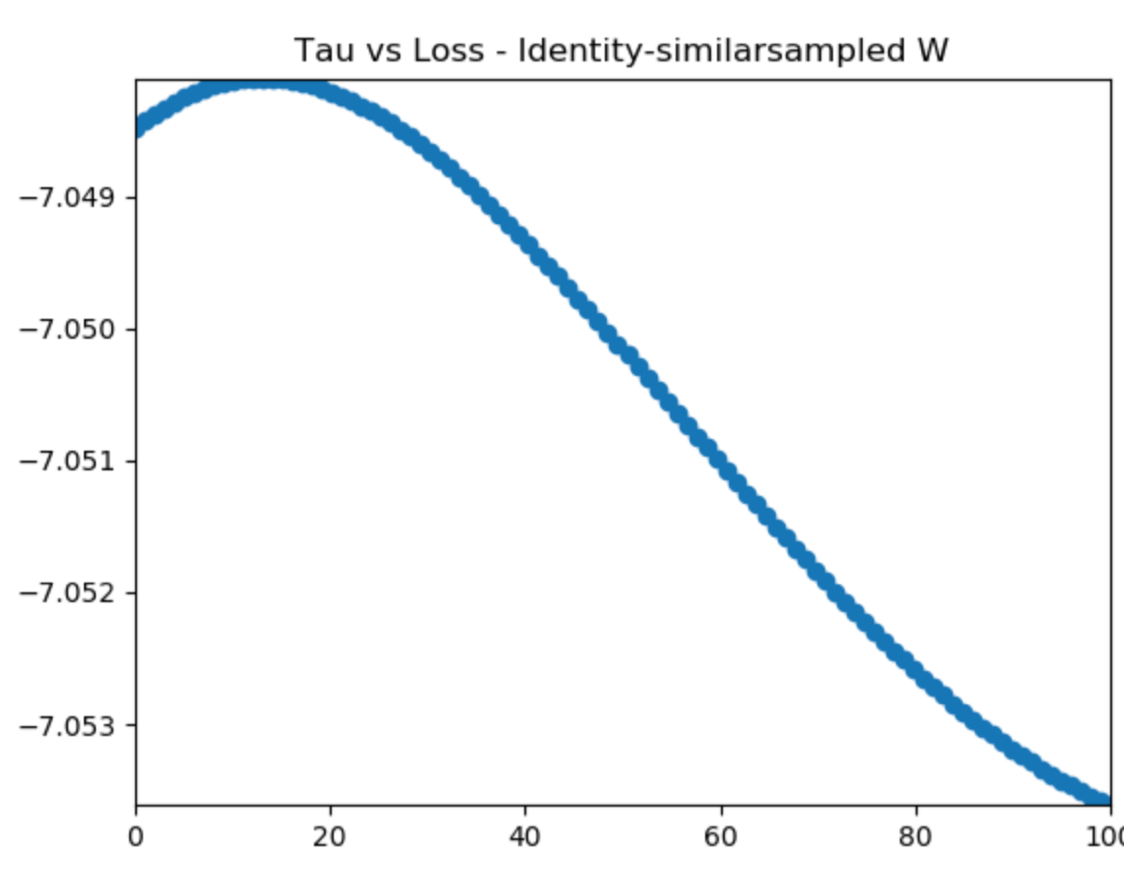
\includegraphics[width=\textwidth]{Appendix1/tau_1}
        \label{fig:tiger}
        \caption{W is taken to be the identity matrix}
    \end{subfigure}   
           \caption{Perturbing $\tau$ and getting a log-likelihood value through $G(\tau)$.
           The function at hand is a Parabola embedded in a 2D space.
           The x-axis refers to the individually sampled $\tau$ values (0 is $\tau = 0$, and 100 is $\tau = 1$ and every value in between is linearly interpolated).
           The y-axis refers to the log-likelihood.
           One can see that the function is smooth on this scale, and that the meaximum is achieved between $0 \leq \tau \leq 0.3 $. }
\end{figure}

\section{Additional Visualization}

The following is a visualization of the sinusoidal function which we use in first part of the quantitave evaluation (i.e. UCB runs):

\begin{figure}[H]
\centering
\begin{subfigure}[b]{0.4\textwidth}
	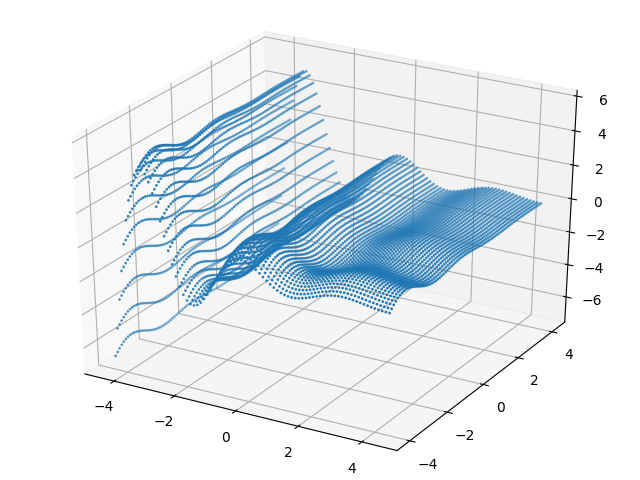
\includegraphics[width=\textwidth]{/visualize_vanillaSinusoidal-5D->2D.png}
	\caption{Sinusoidal used for UCB analysis}
\end{subfigure}
\end{figure}

The above visualization is in contrast to the function which I use in the second part of the quantitative analysis (measuring development of angle loss and log-likelihood), which I present below.
The difference between the two functions is the embeddings, which naturally capture a different range.
However, the embedding is different, and was thus easy to find by Tripathy's method.
This is the same function whose angle Tripathy's algorithm tries to find in chapter 6.

% SINUSOIDAL FUNCTION
\begin{figure}[H]
    \centering
    \begin{subfigure}[b]{0.25\textwidth}
        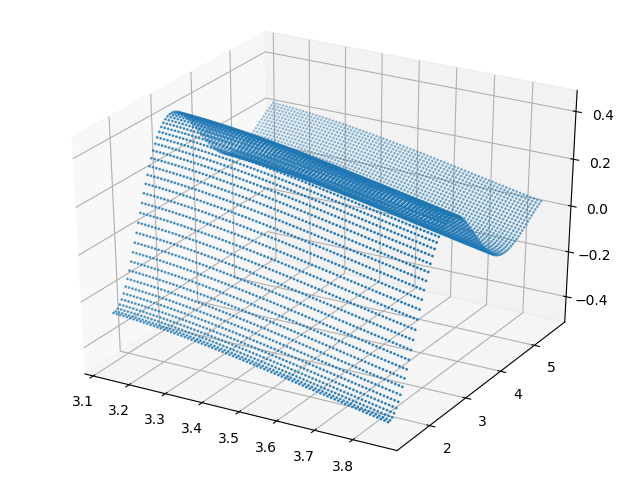
\includegraphics[width=\textwidth]{orig/Sinusoidal-5D-_2D.png}
        \caption{Sinusoidal Original}
        \label{fig:gull}
    \end{subfigure}
    ~ %add desired spacing between images, e. g. ~, \quad, \qquad, \hfill etc. 
      %(or a blank line to force the subfigure onto a new line)
    \begin{subfigure}[b]{0.25\textwidth}
        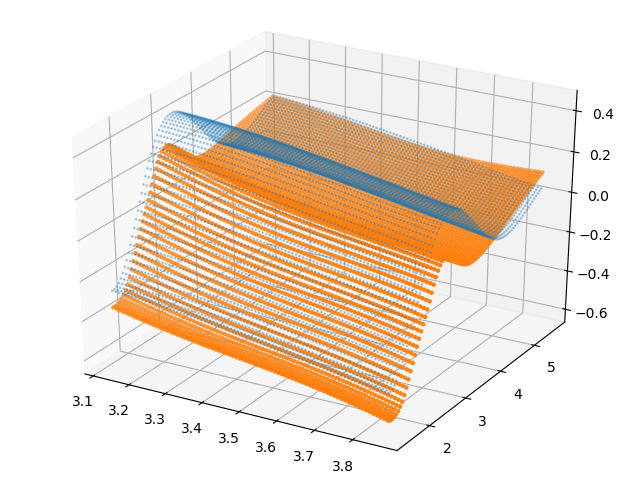
\includegraphics[width=\textwidth]{orig/Sinusoidal-5D-_2D_BORING.png}
        \caption{Sinusoidal Boring}
        \label{fig:tiger}
    \end{subfigure}
        \vskip\baselineskip
 %add desired spacing between images, e. g. ~, \quad, \qquad, \hfill, etc. 
    %(or a blank line to force the subfigure onto a new line)
    \begin{subfigure}[b]{0.25\textwidth}
        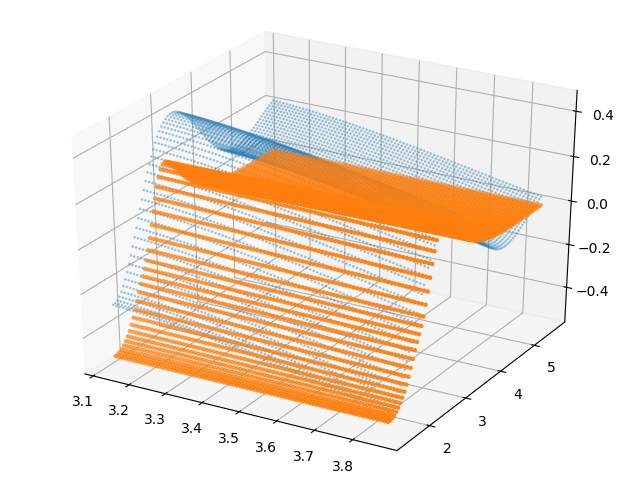
\includegraphics[width=\textwidth]{orig/Sinusoidal-5D-_2D_TRIPATHY.png}
        \caption{Sinusoidal Tripathy}
        \label{fig:mouse}
    \end{subfigure}
        ~ %add desired spacing between images, e. g. ~, \quad, \qquad, \hfill etc. 
    %(or a blank line to force the subfigure onto a new line)
    \begin{subfigure}[b]{0.25\textwidth}
        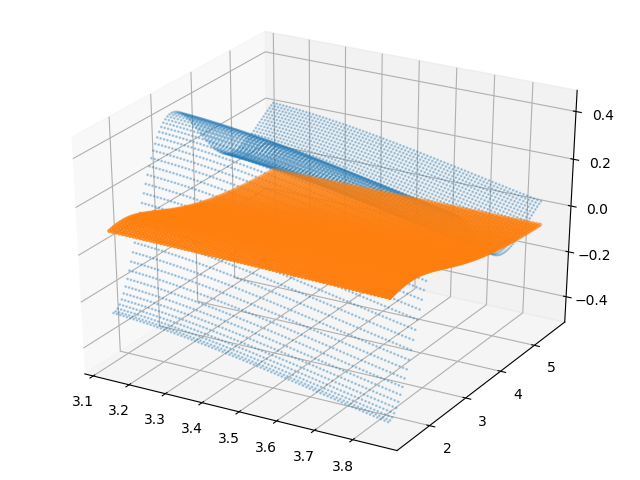
\includegraphics[width=\textwidth]{orig/Sinusoidal-5D-_2D_REMBO.png}
        \caption{Sinusoidal Rembo}
        \label{fig:mouse}
    \end{subfigure}
    \caption{Top-Left: The 2D Sinusoidal-Exponential Function which is embedded in a 5D space.}\label{fig:animals}
\end{figure}

I set the number of restarts to $28$ and number of randomly sampled data points to 100.
The active subspace projection matrix is of size $\mathbf{R}^{1\times 5}$, as this is a function that exhibits a strong principal component, but that still attains small perturbations among a different dimension.
One can see very well here, that BORING can take into account the small perturbations, at a considerably lower cost than Tripathy would be able to.

